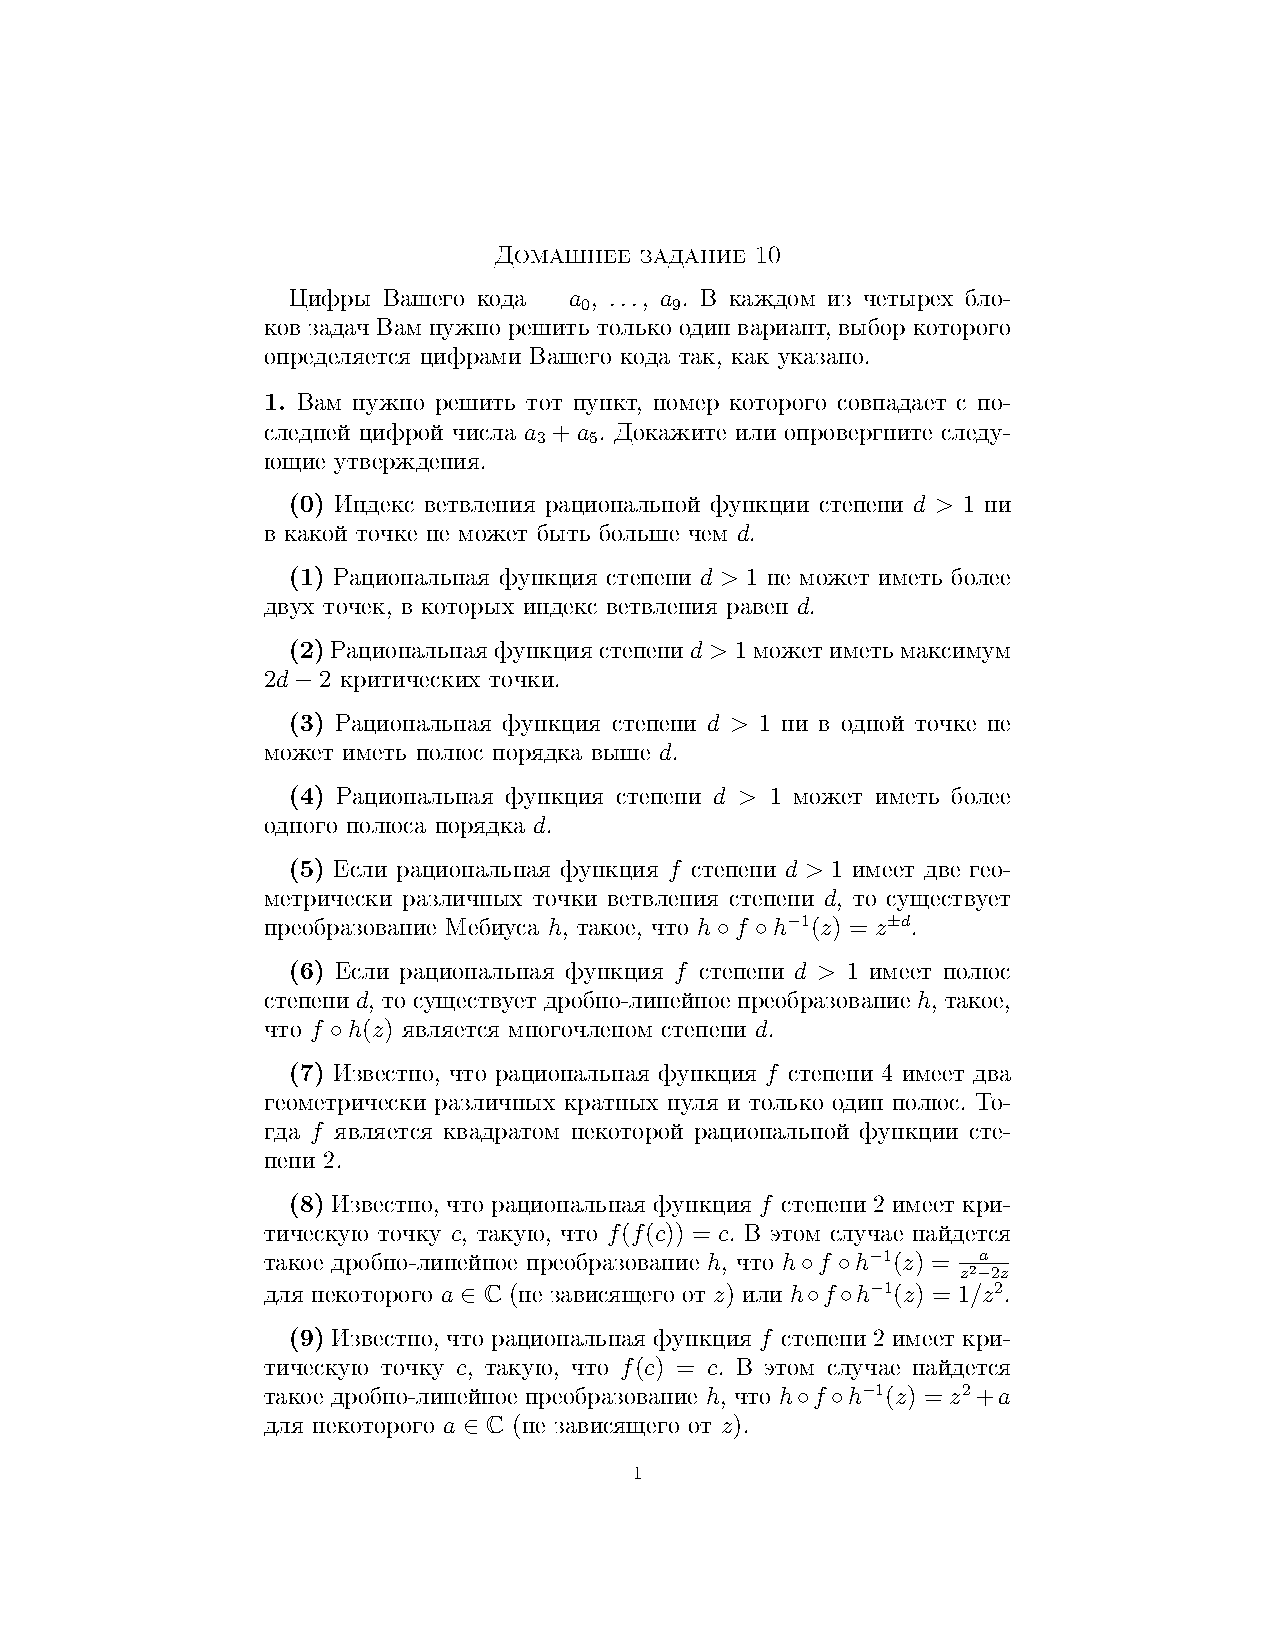
\includepdf[scale=1,pages=1-4]{Tasks/hw10}
\newpage
\section*{Решения}
\subsection*{Задача 1}
	Необходимо решить задачу $a_3 + a_5 = 9 + 6 = 5 \mod 10$\\
	5 задача оказалась сложной, поэтому я записал 4\\
	Заметим что рациональную функцию можно представить в виде $\frac{p(z)}{q(z)}$, допустим что у рассматриваемой функции есть хотя бы 2 полюса степени $d$, назовем их $z_1,\ z_2$. Тогда функцию можно представить как $\frac{p(z)}{(z - z_1)^d (z - z_2)^d q_1(z)}$, $(z - z_1)^d (z - z_2)^d q_1(z) = q(z)$, тогда $\deg((z - z_1)^d (z - z_2)^d q_1(z)) \geqslant 2d$, но $\deg(q(z)) \leqslant d$, противоречие.
\vskip 0.4in

\subsection*{Задача 2}
	Необходимо решить задачу $a_4 + a_6 = 7 + 9 = 6 \mod 10$\\
	\begin{gather*}
		a:\ z \mapsto \frac{z|z|}{1+|z|}\\
		P:\ z \mapsto z^2\\
		b:\ \text{id}\\
		a \circ P \circ b = \frac{z^2|z|^2}{1+|z|^2}
	\end{gather*}
\vskip 0.4in

\subsection*{Задача 3}
	Необходимо решить задачу $a_1 + a_5 = 7 + 6 = 3 \mod 10$\\
	Заметим что $f$ голоморфна, а следовательно аналитична, откуда следует что так как $\mathbb{D} \subset \mathbb{C}$ открыто, то $f(\mathbb{D})$ либо открыта в $\mathbb{C}$, либо константа, рассмотрим $f(z) = C$, $\Re(f(\mathbb{D})) = \Re(C) = \Re(a + bi) = a$, а точка не является открытым множеством
\vskip 0.4in

\subsection*{Задача 4}
	Необходимо решить задачу $a_0 + a_7 = 1 + 3 = 4 \mod 10$\\
	Заметим что функция $\sinh (ax)$ симметрична относительна начала координат
	\begin{gather*}
		\int_{\gamma_{R}} \frac{\sinh (a z) e^{i t z}}{\sinh (b z)} d z=2 \pi i \sum_{1 \leq n \leq R b / \pi} \operatorname{Res}\left(\frac{\sinh (a z) e^{i t z}}{\sinh (b z)}, \frac{\pi i n}{b}\right)\\
	\end{gather*}
	Где $\gamma_{R}$ -- замкнутый контур, состоящий из полуокружности радиуса $R$ и интервала $[-R,R]$, рассмотрев $R \to +\infty$ получим:
	\begin{gather*}
		\int_{-\infty}^{+\infty} \frac{\sinh (a x)}{\sinh (b x)} e^{i t x} d x
		= 2 \pi i \sum_{n=1}^{\infty} \operatorname{Res}\left(\frac{\sinh (a z) e^{i t z}}{\sinh (b z)}, \frac{\pi i n}{b}\right) \\
		= \frac{2 \pi i}{b} \sum_{n=1}^{\infty} \frac{\sinh (a \pi i n / b) e^{-\pi n t / b}}{\cosh (\pi i n)}
		= -\frac{2 \pi}{b} \sum_{n=1}^{\infty}(-1)^{n} \sin (a \pi n / b) e^{-\pi n t / b} \\
		= -\frac{2 \pi}{b} \operatorname{Im}\left(\sum_{n=1}^{\infty}(-1)^{n} e^{\pi n(-t+i a) / b}\right)
		= -\frac{2 \pi}{b} \operatorname{Im}\left(\frac{1}{1+e^{\pi(i a+t) / b}}\right)
	\end{gather*}
	Тогда рассмотрим $t \to 0^{+}$
	\begin{gather*}
		\int_{0}^{\infty} \frac{\sinh(ax)}{\sinh(bx)}dx = \frac{\pi}{2b} \cdot \frac{\sin(a\pi / b)}{\cos(a\pi /b) + 1}
	\end{gather*}
	Откуда при $b = \pi$ получаем
	\begin{gather*}
		\frac{\pi}{2b} \cdot \frac{\sin(a\pi / b)}{\cos(a\pi /b) + 1}
		= \frac{1}{2} \cdot \frac{\sin(a)}{\cos(a) + 1}
		= \frac{1}{2}\tan \frac{a}{2}
	\end{gather*}